\documentclass{article}

% Some useful packages.
\usepackage{amsmath}
\usepackage{siunitx}
\usepackage{graphicx}
\usepackage{verbatim}
\usepackage{mhchem}
\usepackage{textcomp}

% Reduces margins substantially.
\usepackage{geometry}
\newgeometry{margin=2.5cm}

% Allows headers and footers.
\usepackage{fancyhdr}
\pagestyle{fancy}
% Get rid of annoying line under header.
\renewcommand{\headrulewidth}{0pt}

\lhead{}
\chead{BTTM8 - CLIMATE MODELLING - USING HADAM3 TO MODEL CLIMATE CHANGE}
\rhead{}
%\lfoot{}
%\cfoot{}
%\rfoot{}

\usepackage[backend=bibtex,style=authoryear,sorting=nyt,dashed=false]{biblatex}
\bibliography{references/references}
\renewcommand*{\nameyeardelim}{\addcomma\space}

%\newcommand{\coo}{\ce{CO2}}

% 2500 words max.
% Table of information about your simulation (as appendix): 10%
% Discussion of climate model: 15%
% Presentation of experimental results: 30%
% Discussion of experiment: 30%
% Use of wider literature: 5%
% General structure: 10%
%
% 1d.p. throughout.
% When a particular result is noted, try to discuss/explain it.

% Rem: \lp
% Analysing_your_runs
% Converting_UM_files
% Course_work_guide
% geogg134merit
% geogg134pass
% Setting_up_your_runs
% marengoInternal
% WG1AR5_ALL_FINAL
% WG1AR5_AnnexI_FINAL
% WG1AR5_Chapter02_FINAL: Observations: Atmosphere and Surface
% WG1AR5_Chapter06_FINAL: Carbon and Other Biogeochemical Cycles
% WG1AR5_Chapter08_FINAL: Anthropogenic and Natural Radiative Forcing
% WG1AR5_Chapter09_FINAL: Evaluation of Climate Models
% WG1AR5_Chapter14_FINAL: Climate Phenomena and their Relevance for Future Regional Climate Change
% WG1AR5_SPM_FINAL
% WG1AR5_TS_FINAL
% SREX-All_FINAL
% ar4_wg1_full_report
% RCP_Guide
% SREX-Ch3-Supplement_FINAL

\begin{document}

\part*{Using HadAM3 to model global and regional effects of increased atmospheric \ce{CO2}}

\section*{Abstract}

From an initial starting point of \SI{346}{ppm} of \ce{CO2}, HadAM3 is used to model three different scenarios: control, instantaneous doubling of \ce{CO2} and a 1\% rise in \ce{CO2} for 70 years. From these scenarios, the Transient Climate Response (TCR) and effective climate sensitivity to \ce{CO2} ($\Delta T^{eff}_{\ce{CO2}}$, ) are calculated, finding values of $TCR = \SI{2.0}{K}$ and $\Delta T^{eff}_{\ce{CO2}} = \SI{2.9}{K}$. The surface temperature and precipitation differences across the globe between the control scenario and the 1\% rise scenario are analysed. The seasonal variation of precipitation and surface temperature over South America are analysed, and compared to the regional section of IPCC AR5 WG I \parencite{ipcc2014wg1}. The local changes over South America of the variables precipitation, surface temperature, Net Primary Productivity (NPP), humidity and soil moisture are analysed in detail. The interdependence of these variables is demonstrated. % TODO, as well as looking into the reasons for this interdependence.

\section{Introduction}

% Layout the groundwork for why studying CO2 is important:
Since 1958 the level of \ce{CO2} in the atmosphere has been monitored at the Mauna Loa observatory in Hawaii \parencite{keeling1976atmospheric}. Its current level now stands at \SI{401}{ppm} (April, 2014), having increased from a value of \SI{315}{ppm} since 1958, which was already over the maximum value of \ce{CO2} that the Earth had seen for the previous \SI{800 000}{years} \parencite{yin2012individual}. It is a well mixed gas, so its value at on location is indicative of its value across the globe, although there are regional variations \parencite{gurney2002towards}. It is a Greenhouse Gas (GHG), meaning that it is mostly transparent to the short-wave radiation incident on the Earth from the Sun, but opaque to the outgoing long-wave radiation, which has the effect of heating up the Earth's surface \parencite{neelin2011climate}. It is ``very likely'' that it is responsible for the recent global rise in temperatures \parencite{ipcc2014wg1}, which in turn are predicted to lead to increased intensity of tropical cyclones \parencite{knutson2010tropical}, droughts \parencite{dai2012increasing} and extreme precipitation events \parencite{shongwe2009projected}. It is therefore of vital importance that its effect on the Earth's climate is studied, so as the consequences of releasing more \ce{CO2} into the atmosphere can be predicted without performing the actual experiment.

\subsection{General circulation models}
% Explain GCMs.
To study the release of \ce{CO2} into the atmosphere, General Circulation Models (GCMs) can be employed. These model the various processes that make up the Earth's dynamic behaviour such as the movements of the atmosphere or the oceans. They typically model these processes using a grid that spans the surface of the Earth, with variables such as temperature and pressure represented at each grid cell. Early GCMs just modelled the atmosphere \parencite{holloway1971simulation}, but as they have developed they have gone on to encompass more of the Earth's systems, such as the oceans, the cryosphere and the biosphere. Indeed, certain large scale climatic modes such as the El ni{\~n}o Southern Oscillation (ENSO) can only be adequately modelled when the coupling between the atmosphere and the ocean is included \parencite{neelin2011climate}. 

As well as modelling more of the Earth's systems, GCMs have also increased in resolution allowing smaller scale phenomena to be modelled. However, there are processes that occur on a scale smaller than the grid size of the models, and to include these processes they must be parameterised. That is, although the process is not modelled explicitly, it is included in the model by use of a parameter which describes its overall behaviour on the scale of the grid cell. An example of this are the parameterisation of cloud microphysics \parencite{walko1995new, neelin2011climate}.

\subsection{Radiative forcing}
% Talk about Radiative Forcing / no longer! and feedbacks.
Any imbalance between the net incoming short-wave solar radiation and the net outgoing long-wave radiation from the Earth is know as a Radiative Forcing (RF), which is measure in \SI{}{W.m^{-2}}. A positive RF will tend to increase the temperature of the planet, whereas a negative one will decrease it. As the amount of \ce{CO2} in the atmosphere increases, it absorbs more of the outgoing long-wave radiation, which leads to a RF. Similar RFs can be defined for other GHGs such as Methane.

%A climate feedback is a response to e.g. an increase in temperature that can either act to further increase the temperature (positive feedback) or decrease the temperature (negative feedback). One example of a climate feedback is snow albedo, which acts as a negative feedback. The mechanism for this is simple: as temperatures decrease, more snow can form, which increases the albedo of the surface, leading to more reflected radiation and a further drop in temperature (vice-versa for an increase). The most significant of these feedbacks it the water vapour feedback, which is a net positive feedback.

% Talk about regional effects and why they're important.
\subsection{Regional effects of increased \ce{CO2}}
\label{sec:regional_effects}
A \SI{2}{K} rise in global surface temperatures cannot be directly experienced by humans; it is on a regional scale that humans will be affected. It is therefore important that the regional effects of increased \ce{CO2} are understood, so that plans can be put in place to mitigate the worst of these effects and changes can be made ahead of time to adapt to the changing environment. The predicted regional effects over South America are detailed in IPCC AR5 WG I \parencite{ipcc2014wg1}. Two findings from that report will be examined in Section \ref{subsec:seasonal_changes}.

The variables within a GCM are interdependent: the amount of precipitation can affect the NPP, which in turn can affect the amount of transpiration, leading to changes in atmospheric water vapour and changes in precipitation. The role of these dependencies will be analysed in the context of South America, where a details consideration of five of these variables is possible as it is large enough to show spatial variation, but small enough (and geographically disconnected) to be considered as a discrete entity.

\section{Methods}

\subsection{Model}

HadAM3 (Hadley Centre Atmospheric Model 3) is the atmospheric component of the model HadCM3, which was developed in the late 1990s \parencite{pope2000impact}. It uses an Eulerian advection scheme. An Arakawa B grid is used, and the horizontal resolution is 2.5\textdegree\,  latitude by 3.5\textdegree\, longitude, which corresponds to grid cells of approximately \SI{280}{km} by \SI{390}{km} at the equator. There are 19 vertical levels and the model employs a hydrostatic vertical coordinate. The model is run on a \SI{30}{minute} timestep.

The land surface scheme is provided by the Met Office Surface Exchange Scheme (MOSES) \parencite{cox1999impact}. MOSES includes a representation of freezing and melting of the soil moisture layer, which leads to better simulation of surface temperatures. It also includes a new formulation of evaporation, which models the dependence of stomatal resistance on temperature, vapour pressure deficit and \ce{CO2}.


\subsection{Scenarios}

Three scenarios are considered in this study: control, instantaneous doubling of \ce{CO2} (2x\ce{CO2}) and 1\% rise in \ce{CO2} per year (1\%/yr). The \ce{CO2} concentration for the control scenario is \SI{374}, and \SI{748} for the 2x\ce{CO2} and 1\%/yr scenarios. A concentration of \SI{374}{ppm} corresponds to approximately 2005 from the Keeling Curve \parencite{keeling1976atmospheric}. HadAM3 does not directly model the ocean, instead the Sea Surface Temperature (SST) was prescribed for all scenarios. The control and 2x\ce{CO2} scenarios were both prescribed with a SST corresponding to a contemporary climate. For the 1\%/yr scenario, HadCM3 was run for \SI{80}{years} with \ce{CO2} levels increasing at 1\% per year, and the SST from this model from years 60-80 was taken as the SST for the 1\%/yr scenario. It should be noted that a 1\% increase year on year will lead to a doubling after \SI{69.7}{years}.  Each of the runs was run for \SI{21}{years} and \SI{1}{month}.

\newpage
\section{Results}

\subsection{Calculation of TCR and $\Delta T^{eff}_{\ce{CO2}}$}

Once three scenarios (control, 1\%/yr and 2x\ce{CO2}) have been run, some global statistics can be calculated that are useful when comparing the results of different models. The first of these is the TCR, which is the difference in global mean temperature between the 1\%/yr and the control scenarios. The calculated value for HadAM3 in this study is TCR = \SI{2.0}{K}. This is in agreement with IPCC AR5 WG I \parencite{ipcc2014wg1}, which finds that the range is 1.0 to \SI{2.5}{K}.

Another useful parameter in comparing the size of response for different models is the climate sensitivity due to \ce{CO2} ($\Delta T_{\ce{CO2}}$), or the surface temperature change that you would see if you doubled \ce{CO2} concentration and let the Earth reach a new equilibrium. Following method B of \textcite{gregory2004new}, the ``effective climate sensitivity'', $\Delta T^{eff}_{\ce{CO2}}$, can be calculated from the TCR and two flux imbalances, one from each of the 2x\ce{CO2} and 1\%/yr scenarios. If the imposed forcing of doubling \ce{CO2} is $F$, and the net forcing after a given time is $N$, then the climate feedback parameter $\alpha$ can be calculated using:

\begin{equation}
    \alpha = \frac{(F - N)}{\Delta T}
    \label{eqn:alpha}
\end{equation}

Here $\Delta T$ is the TCR already calculated, $F$ is calculated from the 2x\ce{CO2} scenario by taking the difference of the net top of atmosphere flux between the scenario and the control scenario. $N$ is calculated in the same way from the 1\%/yr scenario, which leads to values of $F = \SI{3.71}{W.m^{-2}}$, and $N = \SI{1.05}{W.m^{-2}}$. This gives a value of $\alpha = \SI{1.30}{W.m^{-2}.K^{-1}}$. The equation for climate sensitivity is:

\begin{equation}
    \Delta T^{eff}_{\ce{CO2}} = \frac{F}{\alpha}
    \label{eqn:delta_t}
\end{equation}

Using this equation with the above number yields $\Delta T^{eff}_{\ce{CO2}} = \SI{2.85}{K}$. This is in reasonable agreement with the range found in IPCC AR5 WG I, which gives the range as 1.5 to \SI{4.5}{K} \parencite{ipcc2014wg1}.

\subsection{Global changes between 1\%/yr and control scenarios}

% Points to mention:
% Temp: Highest over Arctic + strongest effect seen in winter. Warning over Antarctic in its winter is far less pronounced.
% only some areas cool at all

% Precip: very different spatial pattern to temp, interesting effect either side of eq. , plus large red. over amazonia DJF visible. Strongest effect in Nov.. 
Figure \ref{fig:global_temp_precip} top-left shows the difference between the 1\%/yr and control scenarios for surface temperature averaged over the year. From this map it is clear that the 1\%/yr scenario is the same temperature or hotter across almost the whole globe. There is only a small area in the Southern Ocean (centred on 60\textdegree S, 120\textdegree E) where the 1\%/yr scenario is cooler. This reflects the value of TCR of \SI{2}{K} found in the previous section. It is also clear from this map that the Arctic shows by far the biggest difference, and this difference is only increased when looking at the northern hemisphere winter December-February (DJF) map, where the difference between the scenarios can reach \SI{20}{K}. However the similar southern hemisphere winter map shows that warming over the Antarctic is far less pronounced. The seasonal dependence of the warming magnitude can be seen in the ``Seasonal mean temperature'' graph, where warming can be seen to be greatest from September to January. The ``Zonal mean temperature'' graph confirms that the heating happens predominantly over the Arctic, with warming being far larger at latitudes higher than 60\textdegree N.

The difference in precipitation between the two scenarios shows a different spatial pattern. In the ``Annual'' map, the main increases can be seen to happen over the Pacific Atlantic and Indian Oceans, just north of the Equator. In the Indian Ocean, there is another area of large increase that can be seen just south of the Equator, and this can be seen as a prominent feature in the ``DJF'' map. The main areas of precipitation reduction are the eastern Pacific Ocean, and over northern Brazil. The reduction over northern Brazil is most prominent in the ``DJF'' map, suggesting a seasonal dependence in this reduction. The ``Seasonal mean precip.'' graph shows a strong increase in November. The ``Zonal mean precip.'' graph shows an increase just north of the Equator, and a corresponding decrease just south of the Equator. There is a broad increase around 50\textdegree S as well.
% TODO: Explain!



\begin{figure}[hbp]
    \centering
    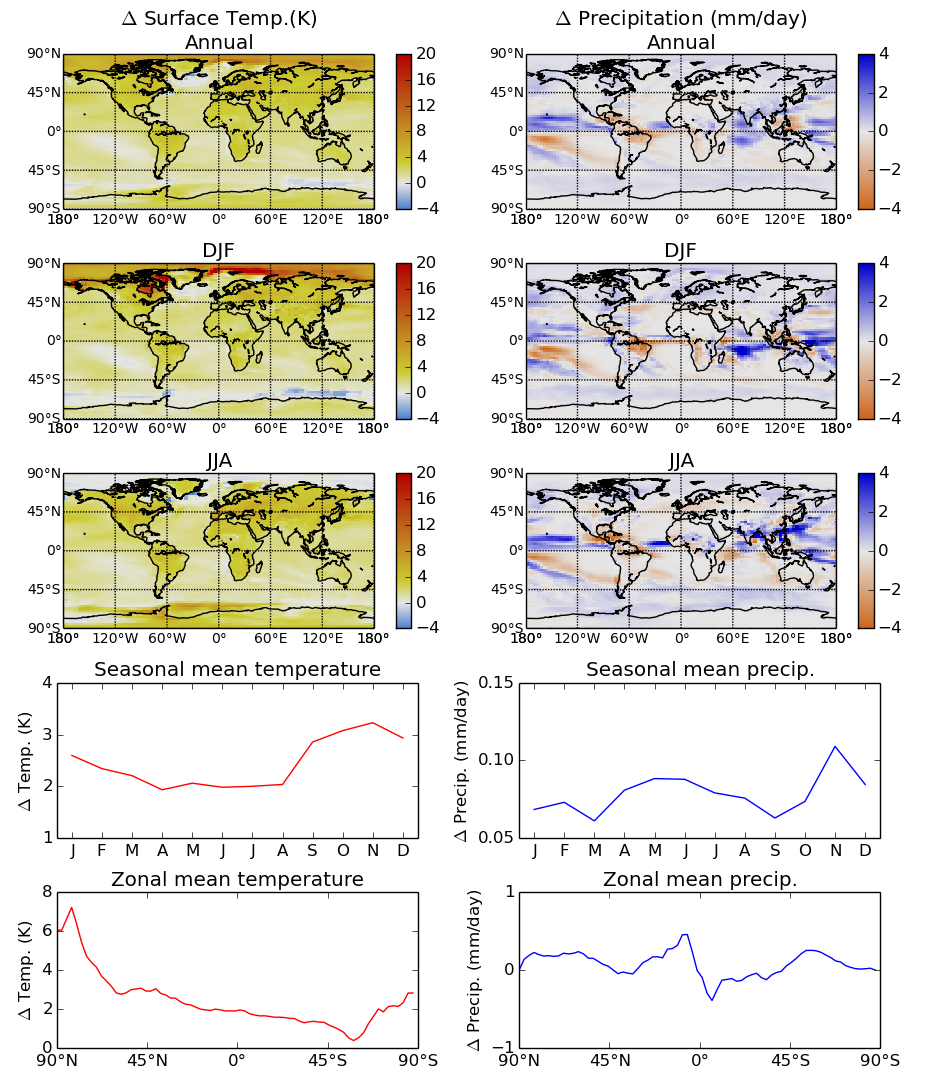
\includegraphics[width=\textwidth]{figures/global_temp_precip}
    \caption{Global annual, December-February (DJF) and June-August (JJA) maps of the difference between the 1\%/yr and control scenarios for surface temperature and precipitation (top three left and right). Seasonal and zonal mean differences between the 1\% and control scenarios for temperature and precipitation (bottom two left and right).}
    \label{fig:global_temp_precip}
\end{figure}

\newpage
\subsection{Seasonal changes in South America}
\label{subsec:seasonal_changes}

% Points to mention:
% precip: Large reduction over amazon in DJF. How this compares to IPCC.
% Large increase over Amazon/North coast of Brazil across the year. Signs of correlation.
From Figure \ref{fig:sa_seasonal}, DJF $\Delta$ Precip. (top left), the same reduction in precipitation over the mouth of the Amazon in northern Brazil that was mentioned in the previous section is clearly visible. This reduction persists across the course of the year (as confirmed in Figure \ref{fig:sa_diff}, top left), although it is most pronounced in DJF. When looking at the change in surface temperature over the same region, the whole of the continent is seen to undergo substantial heating. The average temperature increase over the land is \SI{3.4}{K}. The heating is, again, most prominent over northern Brazil, at the mouth of the Amazon.

\begin{figure}[hbp]
    \centering
    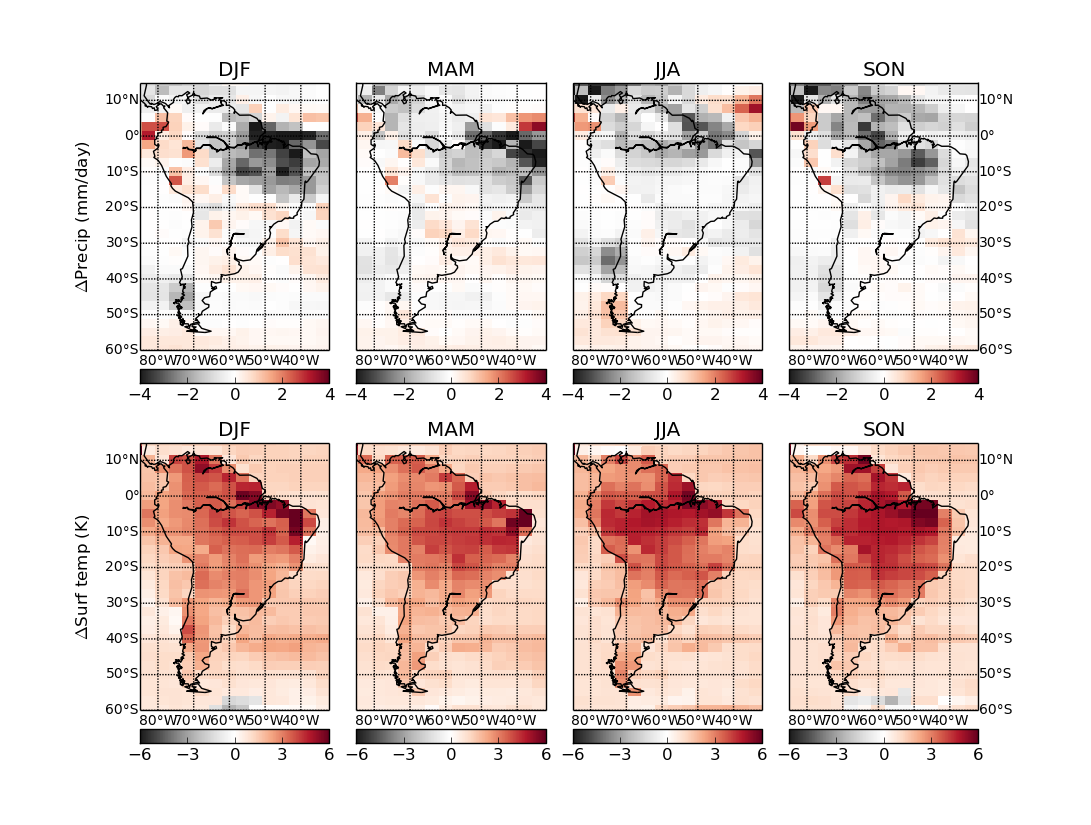
\includegraphics[width=\textwidth]{figures/sa_seasonal}
    \caption{Seasonal variation of the difference between the 1\%/yr and control scenarios for precipitation and surface temperature for South America.}
    \label{fig:sa_seasonal}
\end{figure}

Two findings from IPCC AR5 WG I \parencite{ipcc2014wg1} are:
\begin{enumerate}
    \item ``it is \textit{very likely} temperatures will increase over the whole continent, with greatest warming projected in southern Amazonia.''
    \item ``It is very likely that less rainfall will occur in eastern Amazonia, northeast and eastern Brazil during the dry season. However, in the rainy season there is medium confidence in the precipitation changes over these regions.''
\end{enumerate}

From the maps in Figure \ref{fig:sa_seasonal}, it is clear that the temperature increases over the first whole continent. Therefore The first part of the first finding is replicated by HadAM3. However, the most warming is seen in the north of the Amazon, not the south as in the IPCC report. This could be because the IPCC report uses higher resolution models, that can better reproduce the spatial variation over continents. It could also be because the IPCC report uses regional models to assist in the modelling of certain regions, which will provide more detail (and it is hoped more accuracy) over specific regions of the Earth.

For the second finding, the dry season in Brazil is best shown by the SON map, which does indeed show a significant reduction in precipitation over eastern Brazil. However, a higher reduction is seen in the DJF map, suggesting that once more the HadAM3 model may not be producing the interior detail of the South American continent.

\newpage

\subsection{Interdependence of variables in South America}

% Points to mention:
% Area most affected for 4/5 seems to be north coast of Br., signs of correlation between these 5 variables. 
In the five variables shown in Figure \ref{fig:sa_diff}, three show a broad continental increase between the 1\%/yr and control scenarios: surface temperature, humidity and NPP. Conversely, precipitation and soil moisture both show decreases over the continent. What is interesting is that each of the variables shows an increase or decrease over the head of the Amazon, which hints at these variables' interdependence on each other. That some these variables should be linked is not surprising: it makes sense \textit{a priori} that if e.g. precipitation goes up between the two scenarios, soil moisture should go up as well. The variables humidity and soil moisture have more than one vertical value, so the mean over the vertical coordinate was taken.

\begin{figure}[hbp]
    \centering
    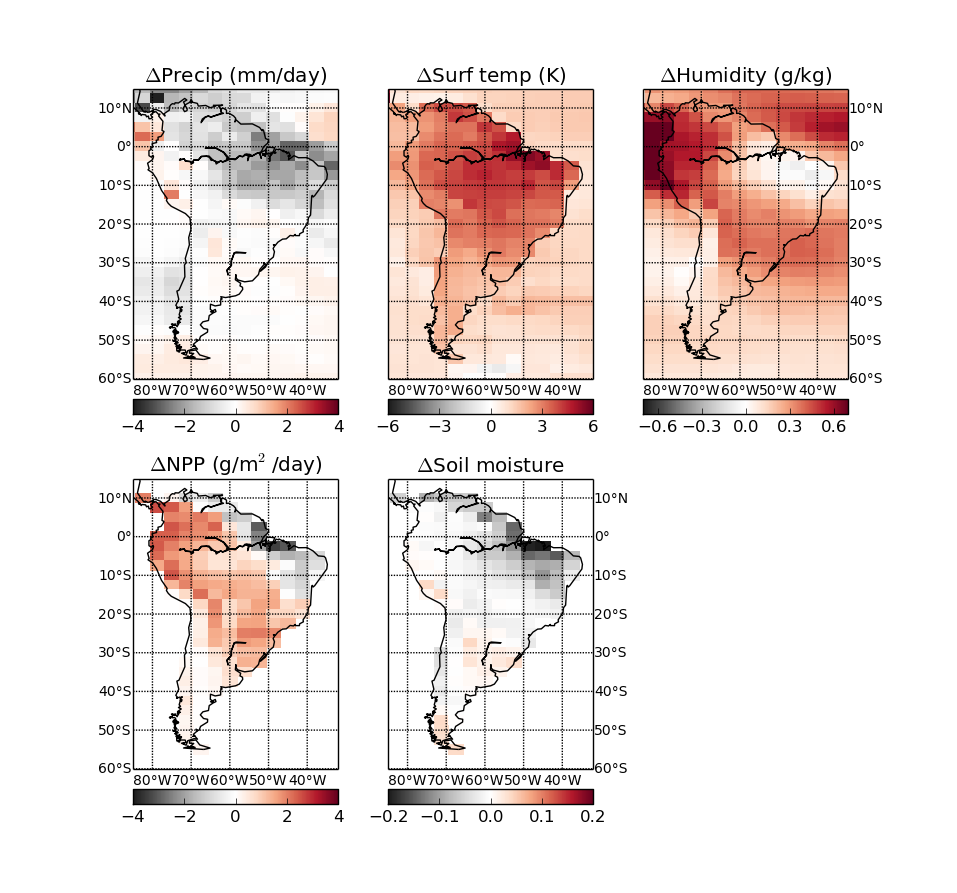
\includegraphics[width=\textwidth]{figures/sa_diff}
    \caption{Annual mean of the difference between the 1\%/yr and control scenarios for precipitation, surface temperature, humidity, NPP, and soil moisture for South America.}
    \label{fig:sa_diff}
\end{figure}

\newpage

% Points to mention:
% Most plots show some amount of correlation (apart from humidity/surf temp.). Implies an interdependency between these variables. explain plausible mechanism for some of these interdependencies. 
This interdependence is examined further in Figure \ref{fig:corr}, which plots the difference of each of the variables between the 1\%/yr and control scenarios against every other variable's difference, showing Pearson's correlation statistic for each pair. This shows that when e.g. there is a strong correlation between the increase in precipitation and the increase in soil moisture between the two scenarios. 

\begin{figure}[hbp]
    \centering
    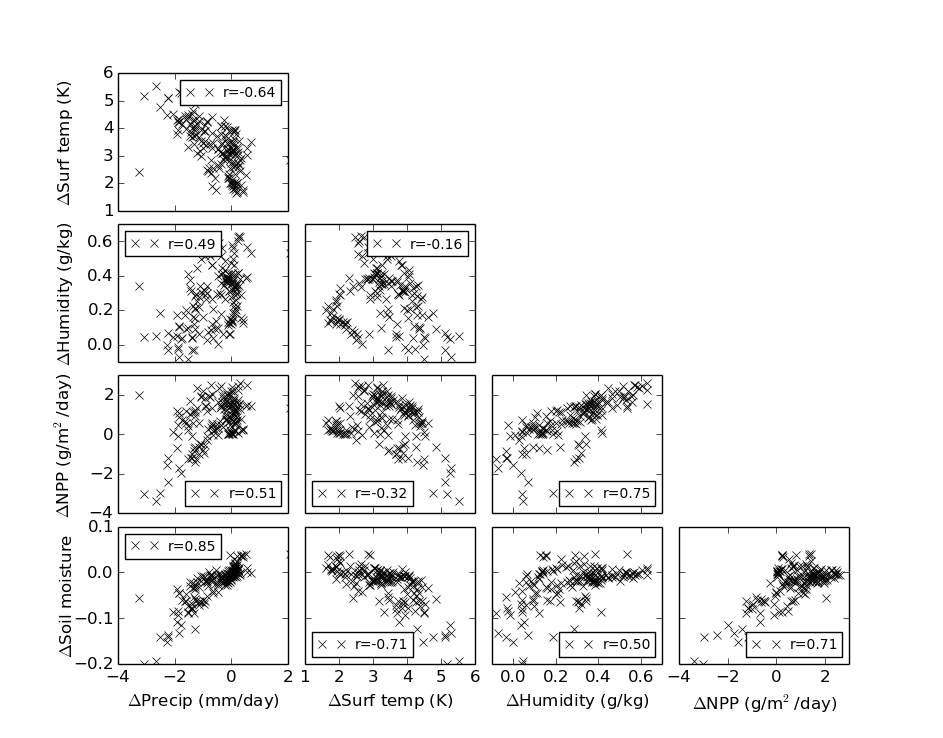
\includegraphics[width=\textwidth]{figures/corr}
    \caption{Scatter plots of the difference between the 1\%/yr and control scenarios for precipitation, surface temperature, humidity, NPP, and soil moisture for South America. Each pair of variables is represented once. Pearson's r value is shown. For all graphs apart from humidity-surface temperature $p < 0.001$, for humidity-surface temperature $p = 0.034$. }
    \label{fig:corr}
\end{figure}

\newpage

\section{Discussion}

The HadAM3 model is 

\section{Conclusions}

Although HadAM3 could not match the predictions of more recent models (as in Section \ref{subsec:seasonal_changes}), it has been used to produce some results that are consistent with the current values, particularly the TCR and the $\Delta T^{eff}_{2x\ce{CO2}}$. Given the low computational cost of running this model - running the model for \SI{21}{years} took about 5 days on a standard computer - makes it well suited for running in a distributed manner across commodity hardware,  as is  being done by climateprediction.net \parencite{stainforth2005uncertainty}. Also, as was done in this study, it can be used to shed light on the interdependence of various variables.

\printbibliography
\appendix 

\section{Additional information}

N.B. more decimal points quoted than required for detailed numerical comparison.

\begin{enumerate}
    \item \textbf{username on \texttt{puma.nerc.ac.uk}}: UCL3
    \item \textbf{simulation id}: xjksa
    \item \textbf{simulation scenario}: 2x\ce{CO2}
    \item \textbf{\ce{CO2} level of scenario}: \SI{692.1}{ppm}
    \item \textbf{global annual average surface temperature}: \SI{277.859}{K}
    \item \textbf{$G_{2x\ce{CO2}}$}: \SI{3.71}{W.m^{-2}}
    \item \textbf{global annual average surface net flux in control}: \SI{10.102}{W.m^{-2}}
    \item \textbf{Transient Climate Response (TCR)}: \SI{2.044}{K}
    \item \textbf{$\Delta T^{eff}_{2x\ce{CO2}}$}: \SI{2.85}{K}
    \item \textbf{RMS surface temperature bias in DJF from control}: \SI{3.943}{K} % TODO: not sure about this one at all.
\end{enumerate}

\end{document}
